	% This is samplepaper.tex, a sample chapter demonstrating the
% LLNCS macro package for Springer Computer Science proceedings;
% Version 2.20 of 2017/10/04
%
\documentclass[runningheads]{llncs}
%
\usepackage{graphicx}
\usepackage{multirow}
\usepackage{amsmath}
\usepackage{caption}
\renewcommand{\arraystretch}{1.2}
% Used for displaying a sample figure. If possible, figure files should
% be included in EPS format.
%
% If you use the hyperref package, please uncomment the following line
% to display URLs in blue roman font according to Springer's eBook style:
% \renewcommand\UrlFont{\color{blue}\rmfamily}

\begin{document}
%
\title{Making History Not Count:\\
Should Historical Corpora Really Be Treated Differently for Event Detection Tasks?}
\titlerunning{Making History Not Count}

%
\titlerunning{Making History Not Count}
% If the paper title is too long for the running head, you can set
% an abbreviated paper title here
%
\author{Andrea Ferretti}
%
\authorrunning{A. Ferretti}
% First names are abbreviated in the running head.
% If there are more than two authors, 'et al.' is used.
%
\institute{University of Milan, Milan, Italy \\
\email{andrea.ferretti1@studenti.unimi.it}}
%
\maketitle              % typeset the header of the contribution
%
\begin{abstract}
The abstract should briefly summarize the contents of the paper in
150--250 words.

\keywords{Event Detection  \and Historical Event Detection \and Glove \and \\ Embeddings comparison.}
\end{abstract}
%
%
%
\section{Introduction}
Word embeddings aim to map words of a vocabulary to vectors of numbers. This is done in order to have a more versatile, tractable, and mathematical representation of those words and improve the performances of several natural language processing tasks. The more intuitive way to do so would be to have a one-hot encoding representation of each word in the vocabulary. This method, however doesn't provide any information about the meaning of a word. To allow the vectors to retain semantic meaning the foundamental idea of distributional semantics is used: words have similar meaning if they appear in similar contexts. This translates to, given a corpus of documents, representing a word as a distribution, over the vocabulary, of the frequency of the words that appear in its context in the corpus. These vectors have the limit of being highly dimensional and extrimely sparse: every word would be represented by a vector of tens of thousands dimensions (the size of the vocabulary) the vast majority of which would have value zero.

To solve these problems several techniques, either based on neural networks or matrix factorization, have been proposed \cite{embeddings}. They both start from the sparse and high dimensional co-occurence matrix and obtain a fixed length, dense, and real valued vector for each word. The vectors are not interpretable when taken singularly, but when analyzed and compared to one another they show interesting properties: words that have similar meaning (in the distributional semantics sense) have vectors that are closed to each other according to the cosine or Euclidean distance, and pairs of vectors representing pairs of words analogy, such as man and woman, king and queen, also have the similar distances. Examples of embeddings algorithms with comparable performance based respectively on neural networks and matrix factorization techniques are Word2Vec \cite{wtv} and GloVe \cite{glove}.

Event detection is one of the numerous tasks that make use of word embeddings. Part of the complexity of the task stems from the intrinsic ambiguity of what can be defined as an event, the Oxford English Dictionary definition of event ``anything that happens, or is contemplated as happening; an incident, occurrence", can be taken as a good baseline. Event detection goes beyond just finding events in unstructured and unprocessed text, it is often concerned with classifying them according to their type and identifying participants and attributes \cite{event-survey1}.

More recently developed event detection systems make heavy use of deep learning techniques, in particular recurrent neural network, in all of its variants, appears to be the more promising model thanks to the possibility of analyzing arbitrarily long sequences of labled data \cite{event-survey2}. Particulary bi-directional long short-term memory (BiLSTM) network appear to be the preferred model.

\section{Research question and methodology}

Most of the efforts in developing event detection systems are focused on contemporary text and on corpora of the biomedical field. The work in \cite{histo} tries to change this by addressing the task of event detection in historical text. It does so by providing a new annotated dataset of events in historical text, a new word embedding created from various historical documents, and a model to detect those events. Starting from these available results, the aim is to both analyze language variation in time and the extent to which this adresses the task of event detection in historical text.

To accomplish the first task the word embedding obtained from historical text of \cite{histo} is compared to a contemporary word embedding, and, in order to have a meaningful baseline, diferrences between two contemporary word embeddings are also taken. There isn't a clear straight forward way to compare word embeddings, but inspired by \cite{embcomp} three methods of analysis are derived. First the distances between pairs of words that are supposed to represent a similar juxtaposition are compared for the embeddings. Then, after having rotated one embedding to best approximate the other \cite{rotation}, the cosine distance of two vectors representing the same words in the two embeddings is calculated. Finally, given a word, the set of k nearset words, according to the cosine distance, is taken for each embedding and the Jaccard distance between the two sets is computed. The rational for all three methods is that the closer are the vectors the more similar are the embeddings.

The set of words chosen for the analysis contains verbs which convey the realization of an event (as described in the event detection guidelines of \cite{histo}), some common words, and words whose meaning is supposed to have evolved or changed during time. Common words are taken as a baseline to measure the distance between other words in the different embeddings.

As for the second task an event detection model based on BiLSTM networks \cite{bilstm} is used. Given two annotated corpora, one historical and one contemporary, each one is split into training and test set, and different combinations of these splits are used to train and evaluate the model to detect event mentions in text (the event classification task is not considered). For example the model can be trained on the training set of the historical corpus and evaluated on the test set of the contemporary corpus. The various results are analyzed to see if there's a substantial difference in performance when changing from historical to contemporary text. The model also takes as a parameter a word embedding: the impact on performances of using a word embedding obtained from historical text opposed to using a word embedding obtained from contemporary text is also analyzed.

\section{Experimental results}

\subsection{Word embeddings comparison}

The word embedding based on historical text (embHisto) is provided by \cite{histo} and is obtained by using the GloVe algorithm on a subset of the Corpus of Historical American English consisting of 36,856 texts published between 1860 and 1939 for a total of more than 198 million tokens. The contemporary embedding (embGlove) is also trained using GloVe on a corpus composed by Wikipedia 2014 and Gigaword 5 for a total of 6 billion tokens. The other contemporary embedding (embCurrent) is also GloVe based and is trained on a subset of Common Crawl corpus for a total of 42 billion tokens. The two contemporary embeddings are provided by \cite{glove} and all three embeddings have vectors of 300 dimensions.

The first method of analysis compares the cosine distance between pairs of words in the various embeddings. The distance function used is the cosine distance because of its invariance to the magnitude of the vectors, accounting only for the angle between them. The underline idea is that juxtapositions should mantain the same distance between each embedding if the relative meaning of the words in the pair is the same. The results are shonw in Table \ref{tab:juxtapos}.

\begin{table}
\centering
\caption{Cosine distances between a pair of words for the various embeddings.}
\label{tab:juxtapos}
\begin{tabular}{|c|c|c|c|}
\hline
\multirow{2}{*}{Word pair} & \multicolumn{3}{|c|}{Cosine distance}\\\cline{2-4}
&embHisto&embGlove&embCurrent\\
\hline
(man, woman) &  0.337 & 0.300 & 0.195\\
(he, she) & 0.283 & 0.292 & 0.130\\
(king, queen) & 0.359 & 0.366 & 0.240\\
(brother, sister) & 0.344 & 0.405 & 0.250\\
(male, female) & 0.198 & 0.105 & 0.062\\
(and, but) & 0.405 & 0.418 & 0.243\\
\hline
\end{tabular}
\end{table}

The second method, given a word, takes the two vectors representing that word in the two embeddings that are compared and computes the cosine distance between those vectors. In order to have a more meaningful comparison, the embeddings should be aligned to compensate for the random position of the vectors in the space \cite{embcomp}, this translates to rotating one embedding to best aproximate the other. This technique exploits the fact that the relative position of many common words is similar across various embeddings, as seen in the previous paragraph. Formalizing the problem we have a matrix $A$ representing the embedding to be rotated, and the matrix $B$ representing the embedding to be aproximate. The matrices, where each row corresponds to a vector of an embedded word, must have the same number of rows and columns, therefore the vocabularies of the embeddings need to be equalized. The solution to how to rotate the matrix is given by the rotation matrix $Q$ obtained by solving the optimization problem know in literature as the orthogonal Procrustes problem:
\begin{align*}
\mathop{argmin}_{\textbf{Q}}\; ||B - AQ|| \\
subject\; to\; QQ^t = I
\end{align*}

After the rotation the cosine distance can be computed. It has been calculated, for the set of chosen words, the distance between the embHisto and embGlove, and the distance between dmbCurrent and embGlove. The results are shown in Table \ref{tab:cosdist}.

The third method compares neighbours, according to the cosine distance, of a word in one embedding to the neighbours of the same word in another embedding. According to the properties of word embeddings, the more similar the embeddings the more similar the neighbours of a word should be. To quantify this similarity, given a word, the set $C$ of words composed of its 100 nearest neighbours in one embedding is used to compute the Jaccard distance with the set of 100 nearest neighbours of that word in another embedding. The Jaccard distance between set $M$ and $N$ is computed as:
\begin{align*}
d_J(M,N) = 1 - { |M \cap N| \over |M \cup N| }
\end{align*}

As before the comparison is done on the same list of words and between the pair of embeddings, after equalizing the vocabularies, embHisto and embGlove, and embCurrent and embGlove. Results are shown in Table \ref{tab:knn}

\begin{table}
\begin{minipage}{.44\linewidth}
\centering
\caption{Cosine distances between words in different embeddings after alignment.}
\label{tab:cosdist}
\begin{tabular}{|c|c|c|}
\hline
\multirow{3}{*}{Word} & \multicolumn{2}{|c|}{Cosine distance}\\\cline{2-3}
&embHisto&embCurrent\\\cline{2-3}
&embGlove&embGlove\\
\hline
did & 0.413 & 0.462\\
does & 0.438 & 0.413\\
do & 0.450 & 0.319\\
be & 0.462 & 0.425\\
is & 0.473 & 0.425\\
make & 0.473 & 0.361\\
made & 0.496 & 0.507\\
have & 0.496 & 0.413\\
had & 0.529 & 0.507\\
but & 0.529 & 0.413\\
and & 0.551 & 0.450\\
done & 0.571 & 0.485\\
get & 0.571 & 0.438\\
were & 0.582 & 0.561\\
got & 0.582 & 0.473\\
was & 0.592 & 0.540\\
has & 0.592 & 0.540\\
makes & 0.667 & 0.507\\
walk & 0.701 & 0.630\\
gets & 0.710 & 0.561\\
hotel & 0.765 & 0.726\\
gun & 0.773 & 0.693\\
airplane & 0.788 & 0.529\\
sport & 0.830 & 0.701\\
fame & 0.837 & 0.639\\
gotten & 0.919 & 0.582\\
sex & 0.930 & 0.851\\
keyboard & 0.985 & 0.684\\
computer & 0.995 & 0.621\\
\hline
\end{tabular}
\end{minipage}
\begin{minipage}{.1\linewidth}
\begin{tabular}{c}
\end{tabular}
\end{minipage}
\begin{minipage}{.44\linewidth}
\centering
\caption{Jaccard distance between sets of neighbours in different embeddings for a given word.}
\label{tab:knn}
\begin{tabular}{|c|c|c|}
\hline
\multirow{3}{*}{Word} & \multicolumn{2}{|c|}{Jaccard distance}\\\cline{2-3}
&embHisto&embCurrent\\\cline{2-3}
&embGlove&embGlove\\
\hline
and & 0.155 & 0.199\\
had & 0.166 & 0.173\\
was & 0.187 & 0.219\\
have & 0.192 & 0.169\\
were & 0.194 & 0.199\\
be & 0.197 & 0.160\\
is & 0.204 & 0.184\\
but & 0.233 & 0.188\\
has & 0.241 & 0.192\\
made & 0.260 & 0.183\\
do & 0.262 & 0.125\\
got & 0.263 & 0.201\\
does & 0.265 & 0.158\\
did & 0.265 & 0.177\\
make & 0.269 & 0.153\\
get & 0.270 & 0.183\\
hotel & 0.289 & 0.307\\
gets & 0.309 & 0.236\\
done & 0.315 & 0.165\\
makes & 0.329 & 0.224\\
walk & 0.332 & 0.229\\
gun & 0.421 & 0.226\\
airplane & 0.452 & 0.224\\
fame & 0.495 & 0.219\\
sport & 0.556 & 0.210\\
sex & 0.567 & 0.310\\
gotten & 0.585 & 0.231\\
keyboard & 0.764 & 0.255\\
computer & 1.076 & 0.174\\
\hline
\end{tabular}
\end{minipage}
\end{table}

\subsection{Event mentions detection}
For the second task of detecting event mentions a BiLSTM network \footnote{https://github.com/UKPLab/emnlp2017-bilstm-cnn-crf}, whose detalied description is given in \cite{bilstm}, is the model used. The complete structure is a bidirectional recurrent neural network that takes as input, encoding the categorical feature as one-hot encoded vectors when needed, the embedding for the word, the lemma of the word, the part of speech, and the casing. These input features are concatenated and fed to a LSTM network composed by two layer of 75 LSTM units each and having a dropout of 0.25 after each layer. The model is bidirectional, meaning there are two LSTM network, one running rom the beginning of the sentence to the end while the other runnig in reverse. The outputs of the two networks are concatenated and fed to a softmax classifier layer.

The datasets used to train the model are the Histo Corpus \cite{histo} \footnote{https://github.com/dhfbk/Histo}, composed of news and travel narratives documents published between the second half of the nineteenth century and the beginning of the twentieth century, and the NIST TAC KBP 2015 Event Nugget Detection corpus \cite{tac} \footnote{https://github.com/UKPLab/tac2015-event-detection/tree/master/tacdata}, composed of contemporary weblogs, broadcast news, newsgroups, broadcast conversation. Event mentions have been manually annotated in the two corpora following different guidelines. Both datasets have been converted to a IOB2 compatible format and they have been divided into a training set and a test set.

The model was trained and evaluated on a subset of the possible combinations (to accomodate the issues given by size disparity of the two corpora) of training sets (trainHisto, trainTAC), test sets (testHisto, testTAC), and two embeddings (embHisto, embGlove). The metrics used for evaluation are precision, recall, and F1-score. Results are shown in table. 



\subsubsection{Sample Heading (Third Level)} Only two levels of
headings should be numbered. Lower level headings remain unnumbered;
they are formatted as run-in headings.

\paragraph{Sample Heading (Fourth Level)}
The contribution should contain no more than four levels of
headings. Table~\ref{tab1} gives a summary of all heading levels.

\begin{table}
\caption{Table captions should be placed above the
tables.}\label{tab1}
\begin{tabular}{|l|l|l|}
\hline
Heading level &  Example & Font size and style\\
\hline
Title (centered) &  {\Large\bfseries Lecture Notes} & 14 point, bold\\
1st-level heading &  {\large\bfseries 1 Introduction} & 12 point, bold\\
2nd-level heading & {\bfseries 2.1 Printing Area} & 10 point, bold\\
3rd-level heading & {\bfseries Run-in Heading in Bold.} Text follows & 10 point, bold\\
4th-level heading & {\itshape Lowest Level Heading.} Text follows & 10 point, italic\\
\hline
\end{tabular}
\end{table}


\noindent Displayed equations are centered and set on a separate
line.
\begin{equation}
x + y = z
\end{equation}
Please try to avoid rasterized images for line-art diagrams and
schemas. Whenever possible, use vector graphics instead (see
Fig.~\ref{fig1}).

\begin{figure}
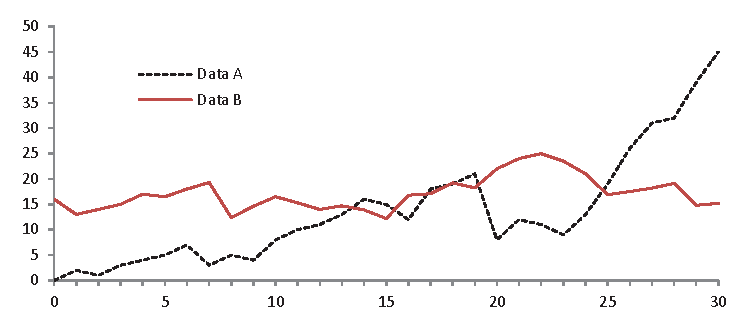
\includegraphics[width=\textwidth]{fig1.eps}
\caption{A figure caption is always placed below the illustration.
Please note that short captions are centered, while long ones are
justified by the macro package automatically.} \label{fig1}
\end{figure}

\begin{theorem}
This is a sample theorem. The run-in heading is set in bold, while
the following text appears in italics. Definitions, lemmas,
propositions, and corollaries are styled the same way.
\end{theorem}
%
% the environments 'definition', 'lemma', 'proposition', 'corollary',
% 'remark', and 'example' are defined in the LLNCS documentclass as well.
%
\begin{proof}
Proofs, examples, and remarks have the initial word in italics,
while the following text appears in normal font.
\end{proof}
For citations of references, we prefer the use of square brackets
and consecutive numbers. Citations using labels or the author/year
convention are also acceptable. The following bibliography provides
a sample reference list with entries for journal
articles~\cite{ref_article1}, an LNCS chapter~\cite{ref_lncs1}, a
book~\cite{ref_book1}, proceedings without editors~\cite{ref_proc1},
and a homepage~\cite{ref_url1}. Multiple citations are grouped
\cite{ref_article1,ref_lncs1,ref_book1},
\cite{ref_article1,ref_book1,ref_proc1,ref_url1}.
%
% ---- Bibliography ----
%
% BibTeX users should specify bibliography style 'splncs04'.
% References will then be sorted and formatted in the correct style.
%
% \bibliographystyle{splncs04}
% \bibliography{mybibliography}
%
\bibliography{biblio}
\bibliographystyle{ieeetr}
%
%\bibitem{ref_article1}
%Author, F.: Article title. Journal \textbf{2}(5), 99--110 (2016)

%\bibitem{ref_lncs1}
%Author, F., Author, S.: Title of a proceedings paper. In: Editor,
%F., Editor, S. (eds.) CONFERENCE 2016, LNCS, vol. 9999, pp. 1--13.
%Springer, Heidelberg (2016). \doi{10.10007/1234567890}

%\bibitem{ref_book1}
%Author, F., Author, S., Author, T.: Book title. 2nd edn. Publisher,
%Location (1999)

%\bibitem{ref_proc1}
%Author, A.-B.: Contribution title. In: 9th International Proceedings
%on Proceedings, pp. 1--2. Publisher, Location (2010)

%\bibitem{ref_url1}
%LNCS Homepage, \url{http://www.springer.com/lncs}. Last accessed 4
%Oct 2017

\end{document}
